%%Main takeaway - we provide calving front locations, and have automated it
%Some may be more interested in the data, or the method, so make sure we cover both

\documentclass[tc, manuscript]{copernicus}

\usepackage{wrapfig}
\usepackage{multirow}
\usepackage{float}
\usepackage{array}
\usepackage{booktabs}
\usepackage[table]{xcolor}
\usepackage[font=small,skip=4pt]{caption}

\begin{document}

\title{Calving Front Machine (CALFIN): A Glacial Termini Dataset and Automated Deep Learning Methodology for Greenland, 1972-2020}

\Author[1]{Daniel}{Cheng}
\Author[1]{Wayne}{Hayes}
\Author[2]{Eric}{Larour}
\Author[1]{Yara}{Mohajerani}
\Author[2]{Michael}{Wood}
\Author[1]{Isabella}{Velicogna}
\Author[1,2]{Eric}{Rignot}

\affil[1]{University of California at Irvine, Irvine CA, USA}
\affil[2]{Jet Propulsion Laboratory, California Institute of Technology, Pasadena CA, USA}

\runningtitle{TEXT}

\runningauthor{TEXT}

\correspondence{Daniel Cheng (dlcheng@uci.edu)}

\received{}
\pubdiscuss{} %% only important for two-stage journals
\revised{}
\accepted{}
\published{}

\maketitle

\begin{abstract}
We present Calving Front Machine (CALFIN), an automated method for extracting calving fronts  from satellite images of marine-terminating glaciers. We present results using Landsat imagery from 1972 to 2019, and generate 20001 calving front lines across 67 Greenlandic glaciers. This method is uniquely robust to clouds, illumination differences, ice mélange, and Landsat-7 Scan Line Corrector errors. The current implementation offers a new opportunity to explore previous sub-seasonal trends, and validate existing models moving forward.

This method utilizes deep learning, and builds on existing work by Mohajerani et al., Zhang et al., and Baumhoer et al. Additional post-processing techniques allow our method to achieve accurate and useful segmentation of raw images into Shapefile outputs. 

CALFIN excels among the current state of the art. We show this by performing a model inter-comparison to evaluate performance against existing methodologies. We also evaluate CALFIN's ability to generalize to SAR imagery. CALFIN's fronts are often indistinguishable from manually-curated fronts, deviating by 2.25 pixels (86.76 meters) from the true front on a diverse set of 162 testing images.
\end{abstract}

\introduction
\label{sec:intro}
The evolution of Greenland's tidewater glaciers is an important constraint on the evolution of the Greenland Ice Sheet as a whole. Likewise, changes in Greenland are important in tracking and predicting changes in the climate overall. Constraining Greenland's glacial evolution is thus an important part of improving our understanding of Earth's changing climate.

One constraint on glacial evolution is the position of glacial calving fronts over time. Currently, most calving front delineation is done with time-consuming manual labor. This results in severe under-coverage of available satellite imagery. As a result, many smaller glaciers have {\em no} calving front data, while others have annual or seasonal coverage at best.

Existing efforts have been made to provide calving front positions. These include ESA-CCI's dataset of 26 Greenlandic glaciers from 1990-2016, PROMICE's dataset of 47 glaciers from 1990-2018, and MEaSUREs' dataset of 200+ glaciers from 2000-2017\citep{enveo2017,andersen2019,Joughin2015}. Additionally, there are many other teams including Bunce et al., Carr et al., Murray et al., and Catania et al. Moreover, there are growing efforts to provide a unified database of manually delineated calving front. Nevertheless, the constant cost of adding of new data - as well as the current lack of spatio-temporal resolution in existing data - implies a consistent need for new data assimilation efforts.

The automation of glacial calving front delineation alleviates these needs. However, confounding issues - such as cloud cover, ice mélange, and shadows - impede naive techniques such as edge detection \citep{paravolidakis2016} and texture analysis \citep{malik2001}. Nonetheless, modern machine learning techniques and deep neural networks provide a robust, scalable, and accurate solution.

In this study, we present novel contributions to automated glacial calving front delineation. We apply our automated methods to Helheim, Kangerlussuaq, Kong Oscar, Hayes, Rink Isbrae, Upernavik, Jakobshavn, Kangiata Nunaata, Petermann, and 58 other nearby Greenlandic glaciers. We use Landsat Near-Infrared band images spanning from 1972 to 2020.

We utilize deep convolutional neural networks to process our source data. We contribute a modified version of the UNet-style DeepLabV3+ Xception network, along with the final network parameters we use for dataset production. We contribute the generated dataset, which consists of Shapefile polyline/polygonal time series, for each of the 67 Greenlandic glacial basins.

We compare our methodology and its results against studies by Mohajerani et al., Zhang et al., and Baumhoer et al.

Our key takeaway is the maturation of neural networks for automated calving front detection. Specifically, a well trained network now approaches human levels of accuracy in picking arbitrary glacial calving fronts - without retraining. This reinforces existing studies on the viability of the methodology, and paves the way for applications on other data assimilation tasks.

Our main goal and contribution is to automatically provide high spatial accuracy, dense temporal resolution, and long time series calving front locations for the cryospheric/climate modeling community.

\section{Data Source and Scope}
\label{sec:datasources}
We begin by evaluating several potential data sources, including Terra/MODIS, TerraSAR-X, Landsat, and Sentinel. We select Landsat for its long time-series availability and reasonable spatial distribution/resolution (see Table \ref{tab:datasources}).

\begin{table}[h]
    \centering
    \caption{A comparison of the data sources available for use.}
    \begin{tabular}{cccccc}
        \hline
        \rowcolor[rgb]{0.71,0.71,0.71} \multicolumn{6}{c}{\textbf{Potential Data Sources}} \\ \hline
        \rowcolor[rgb]{0.71,0.71,0.71} Name & Resolution(s) & Time Series & Repeat Cycle & Sensor & Seasonal Coverage \\ \hline\hline
        Landsat & 30m, 60m & 1972-present & 16 day & Optical & Spring-Fall \\ \hline
        \rowcolor[rgb]{0.886,0.886,0.886} Terra (MODIS) & 250m, 500m, 1000m & 1999-present & 1, 8, 16 day & Optical & Spring-Fall \\ \hline
        Sentinel & 10m, 20m, 60m & 2014-present & 10, 12 day & SAR & Spring-Winter\\ \hline
        \rowcolor[rgb]{0.886,0.886,0.886} TerraSAR-X & 1m, 3m, 6m & 2007-present & 3-11 day & SAR & Spring-Winter\\ \hline
    \end{tabular}
    \label{tab:datasources}
\end{table}

With Landsat as our data source, we can define CAFLIN's spatial extent and time series coverage. We provide calving fronts for 67 Greenlandic basins, spanning the period from 1972 to 2020. Basins are selected for their high drainage volume and wide spatial distribution.

We provide the full spatial coverage map (Figure \ref{fig:spatial_coverage}) and temporal coverage chart for 8 high drainage volume basins (Figure \ref{fig:temporal_coverage}).  For the full temporal coverage chart showing all 67 basins, see the attached Supplement.

\begin{figure}[h]
    \centering
    \begin{minipage}{10.5cm}
        \centering
        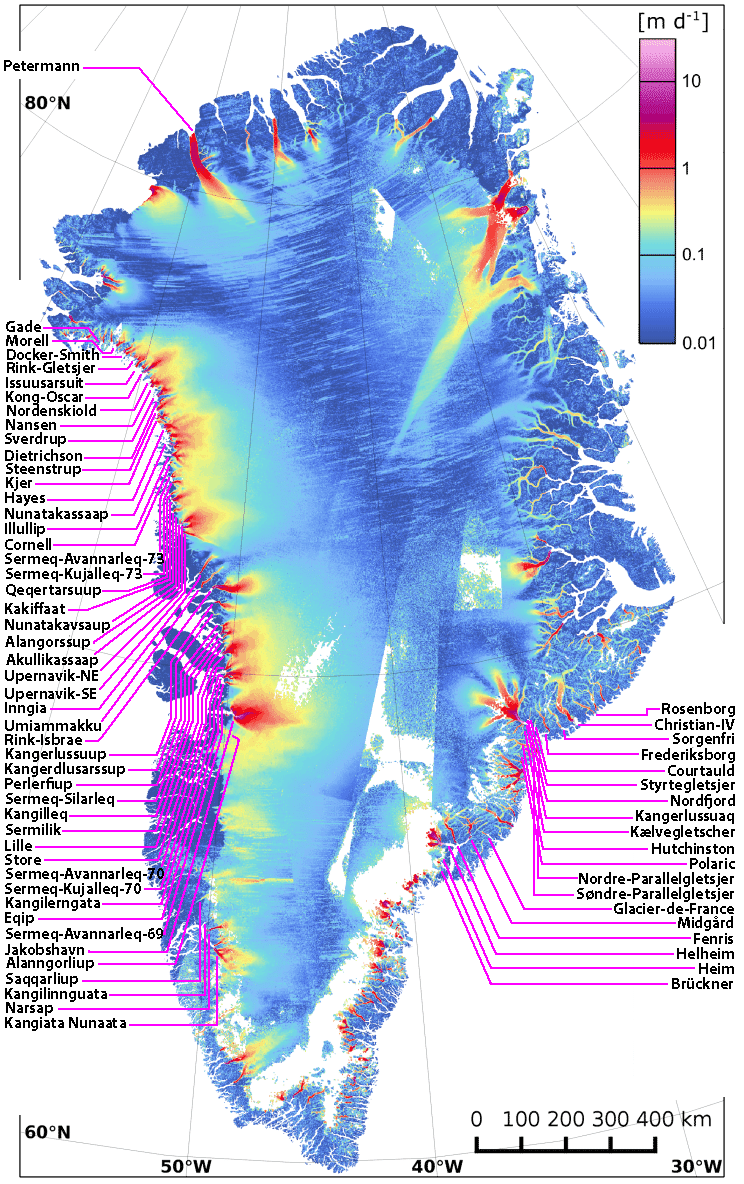
\includegraphics[width=10.5cm]{figures/spatial_66.png}
        \caption{Spatial distribution of 67 Greenlandic glaciers. We study glaciers with reasonable drainage volumes and wide spatial distribution. Velocity map taken from Nagler \citep{nagler2015}.}
        \label{fig:spatial_coverage}
    \end{minipage}
    \hspace{0.5cm}
    \begin{minipage}{6cm}
        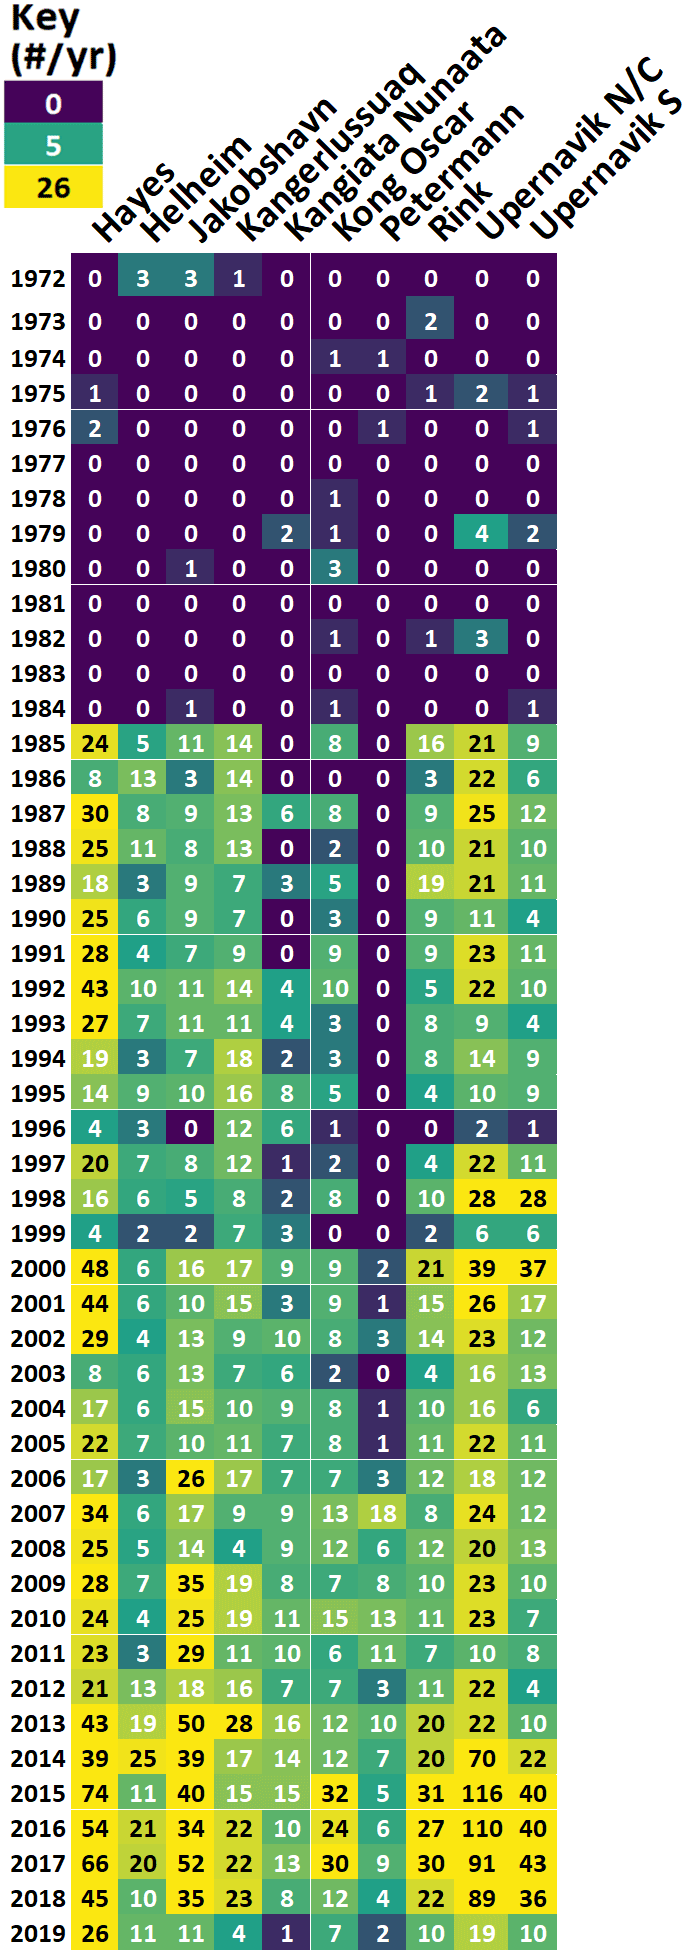
\includegraphics[width=6cm]{figures/temporal.png}
        \caption{Number of images across the years for 8 selected glaciers.}
        \label{fig:temporal_coverage}
    \end{minipage}
\end{figure}

\section{Methodology}
\label{sec:method}
\subsection{Preprocessing}
\label{sec:preproc}
We develop a pipeline (Figure \ref{fig:preprocess}) that automates much of the data preprocessing that prepares raw data for input into the neural network.

\begin{figure}[h]
    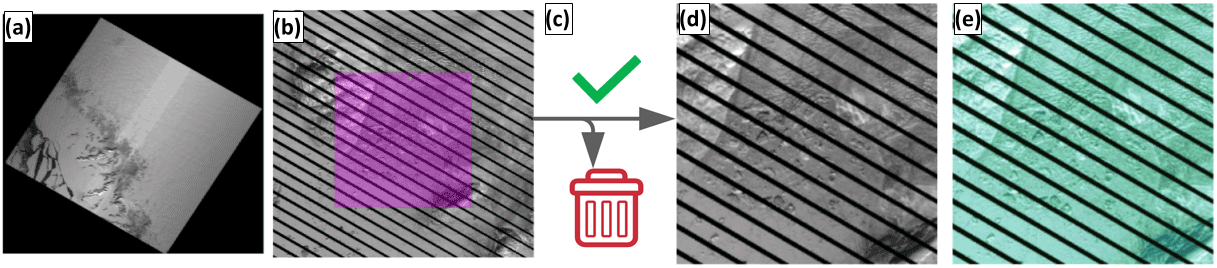
\includegraphics[width=14cm]{figures/pipeline-preprocess.png}
    \centering
    \caption{A visual outline of preprocessing steps.}
    \label{fig:preprocess}
\end{figure}

We first collect all input raster images centered around one of 9 primary glacial basins. These basins include Kong Oscar, Hayes, Rink Isbrae, Upernavik, Jakobshavn, Kangiata Nunaata, Helheim, Kangerlussuaq, and Petermann. We select all L1TP (precision and terrain corrected) rasters from Landsats 1-8 with low cloud coverage (\textless20\%). We add selected L1GS/L1GT (non-corrected) products, which we manually georeference, to fill in Landsat 1-2 time series gaps (1972-1985). At this stage, we accumulate a total of 4956 Landsat rasters.

To begin subsetting, we define the domain of a glacial basin as a rectangular Shapefile polygon, which enclose the expected  range of calving front locations.

After subsetting, we automatically prune images that are ill-suited for further processing. We remove subsets that contain \textgreater30\% NODATA pixels, or \textgreater20\% cloud pixels. This allows us to process images with Landsat 7 scan-line errors and domains along raster boundaries, while still filtering out largely out-of-bounds subsets. At this stage, We accumulate 20188 GeoTIFF subsets.

We then convert the subsets from their native GeoTIFF formats to a standardized 256x256 PNG image.

Lastly, we utilize two detail enhancements to allow for better detection for images with low contrast or heavy shadows. We currently use the Pseudo-HDR Toning and Shadows/Highlights enhancements from Adobe Photoshop. We stack the raw, HDR, and S/H enhancements into a single RGB image. 

At this point, the images are ready for processing into calving front masks.

\subsection{Neural Network Processing}
\label{sec:proc}
Images are processed using the Calving Front Machine Neural Network (CALFIN-NN). As a neural network, CALFIN-NN works like an advanced k-NN or SVM classifier, only with higher order kernels that are automatically computed during the training process. Once trained, CALFIN-NN takes in images, and outputs masks that classify each pixel based on their probability of lying on the coastline/calving front. CALFIN-NN also generates a land/ice-ocean mask as a secondary output. Once each image is processed, the calving front is ready to be extracted during post-processing.

\begin{figure}[h]
    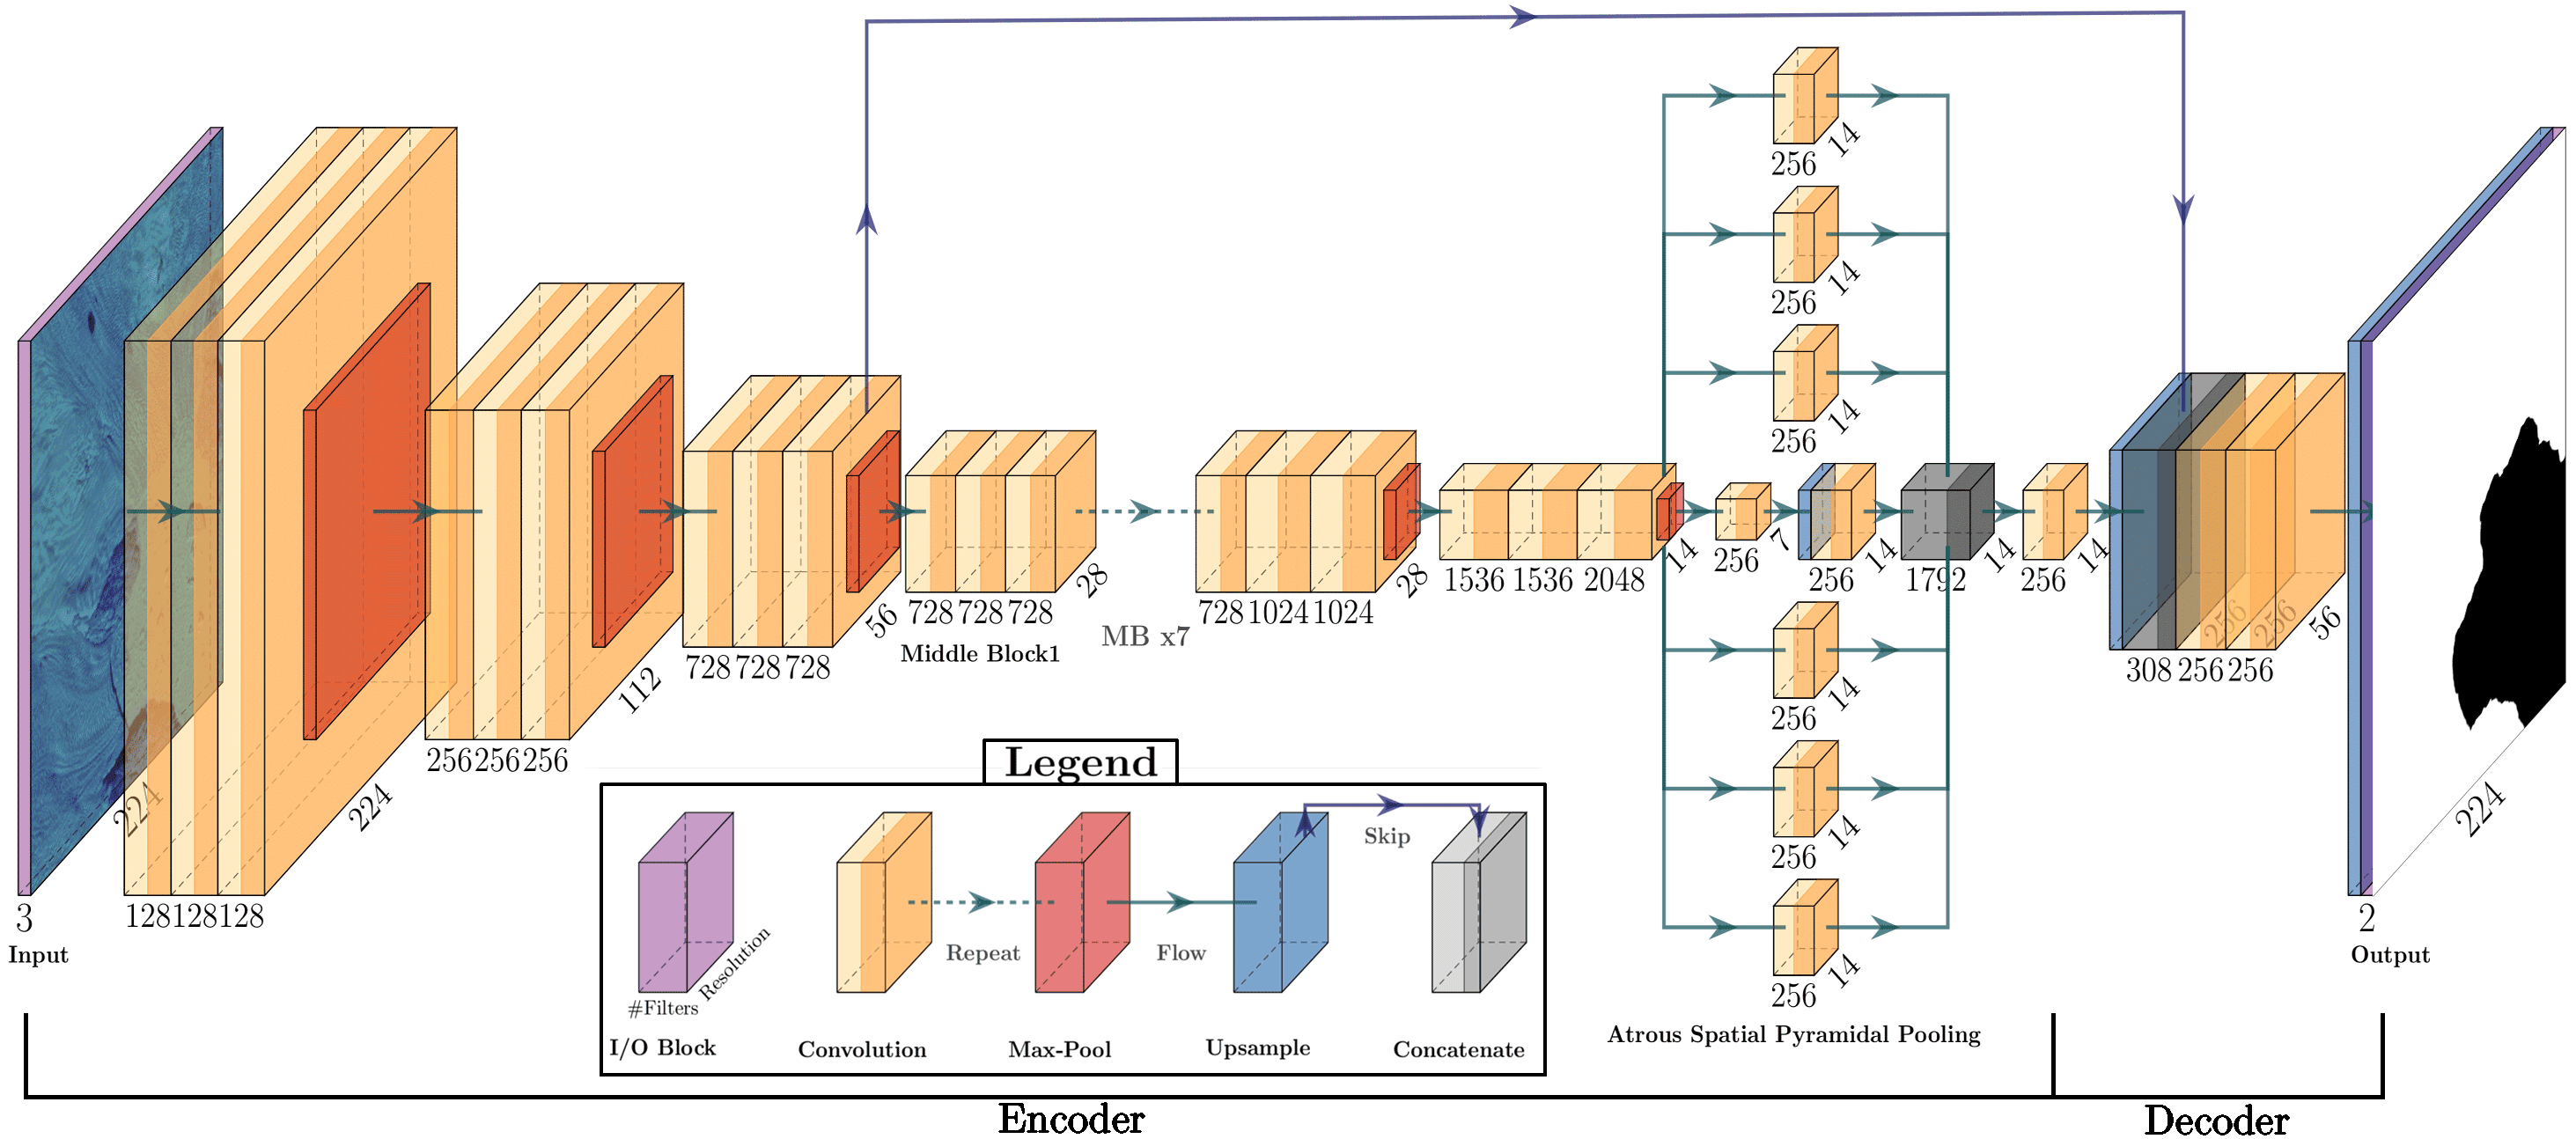
\includegraphics[width=16cm]{figures/arch_final.png}
    \centering
    \caption{CALFIN-NN processing architecture. Each orange "Xception" block consists of convolution kernels that detect basic features in the previous block. To balance increasingly complex and numerous feature maps, the size is halved periodically. "U" shaped connections help refine the localize the masks as they are re-scaled to their original size. Note that the 7 repeated "Xception" blocks in the middle section have been omitted for brevity.}
    \label{fig:NNarch}
\end{figure}

\subsubsection{Network Architecture \& Modifications}
\label{sec:arch}
The following section goes into additional detail regarding aspects of our neural network model. Further details - including the iterative design process and our final training regimen - are described in Discussion. 

CALFIN-NN inherits from the U-Net family of image segmentation architectures. Thus it is capable of learning abstract image features, and outputting confidence masks where it detects ice, ocean, and calving fronts. Most importantly, neural networks like CALFIN-NN generalize to new data automatically. This key capability is the foundation of most other automated methods in this field \citep{zhang2019, mohajerani2019, baumhoer2019}.

We build upon this work, and utilize a modification of Google's DeepLabV3+ Xception \citep{chen2018} image segmentation network. This modified network architecture is shown in Figure \ref{fig:NNarch}. 

The first half of the network - the encoder - uses the Xception-65 network \citep{chollet2016} as our feature extractor. These features encode information in the image using higher-order image kernels. In other words, it assembles basic features (such as edges, corners) into more abstract features (such as glacier/land textures). DeepLabV3+ adds in a Atrous Spatial Pyramidal Pooling (ASPP) module that further enhances multi-scale feature detection, as each separate block in the ASPP module uses kernels dilated to a different scale.
The second half of the network - the decoder - takes the output of the encoder and the ASPP module, up-samples the features and predicts the final output before performing one last up-sampling to the original input/output size. Note the usage of 4x instead of 2x up-sampling, common in traditional  We found that there was no significant decrease in performance when using 4x up-sampling, which is consistent with the findings in the DeepLabV3+ paper\citep{chen2018}.

We make several modifications to the basic DeepLabV3+ Xception model architecture. We add additional Atrous Spatial Pyramidal Pooling (ASPP) blocks with different dilation scales (6, 12, 18 in the original, compared to 1, 2, 3, 4, 5 in CALFIN-NN) to more accurately recognize thin/line like features such as calving fronts. We also modify the deepest pooling layer to only down-sample by 2 instead of 14, to preserve the feature localization. We reduce the number of Middle Blocks (MB in Figure 4) from 16 to 8, as we do not need the extra discriminative power that such blocks would offer. Together, these changes account for differences in input size when compared to the original model (224 vs 512) and enable better multi-scale feature localization. We switch the encoder module from the Xception 71 layer model to the Xception 65 layer model and remove the header module of DeepLabV3+, as both reduced the resolution of the image too much for accurate edge localization. We also modified tail of the network to output 2 channels for mask and edge simultaneously. These changes both reduce the weight size from ~40m parameters to ~29m parameters (~400MB on disk) as well as increase the overall accuracy of the network.

Altogether, these novel capabilities advance the state-of-the-art in image segmentation within the cryosphere community.

\subsection{Post-Processing}
\label{sec:postproc}
At this stage, the 2-channel pixel mask output of CALFIN-NN is post-processed to extract useful Shapefile data products. There are several steps with non -trivial solutions, which we cover in the following subsections. See Figure \ref{fig:postproc} for a visual outline of these steps.

\begin{figure}[h]
    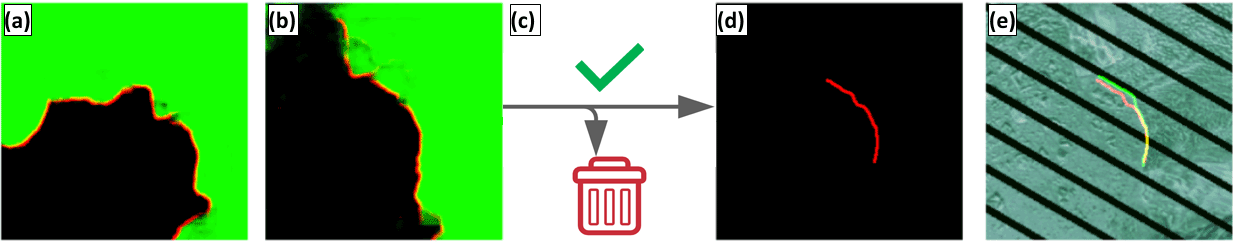
\includegraphics[width=14cm]{figures/pipeline-postprocess.png}
    \centering
    \caption{A visual outline of post-processing steps. Note that steps 2-5 may be repeated multiple times if multiple fronts are detected.}
    \label{fig:postproc}
\end{figure}

\subsubsection{Calving Front Reprocessing}
\label{sec:reproc}
We first isolate individual fronts from the processed image and reprocess subsets of the input image wherever they are detected. The front detection method is described in Section \ref{sec:coastline}. We also exploit the nature of CALFIN-NN's output as a confidence measure, so that generated fronts can be filtered out based on classification confidence thresholds.

\subsubsection{Pixel Mask to Coastal Polyline}
\label{sec:pixel_mask}
Next, we fit a polyline to the pixel mask to retrieve the correct coastline boundary. The line fitting algorithm shares similarities to point cloud to line approximation methods \citep{zolnieruk2016}. Our algorithm is implemented by converting each pixel in the mask to nodes in a graph, and finding the single longest path in the graph's minimum spanning tree.

The algorithm begins by calculating the euclidean distances between each node and every other node, creating distance matrix D. 
Then for each point, find the k-nearest neighbors graph using distance matrix D. This ensures a connected path with continuous lines, while still allowing for large gaps in the pixel mask to be crossed. K is empirically chosen to be the maximum of some minimum number of nodes (we choose 4) and some percentage of the total number of nodes (we choose 20\%). 
Now, we remove outliers by using the robust Modified Z-score method with Median Absolute Deviation \citep{garcia2012}. We eliminate any node whose mean neighbor distance exceeds a Z-score of 10. 
Next, we use the k-nearest neighbors graph to construct a undirected weighted minimum spanning tree (MST). Lastly, we find the longest path in the MST. This can be done by performing 2 depth-first searches (DFS), with each DFS finding one endpoint along the longest overall path. This path corresponds to the coastal polyline detected by CALFIN-NN.

\subsubsection{Coastline to Calving Front}
\label{sec:coastline}
Next, we isolate the calving front from the coastline polyline. We utilize fjord boundary masks created for each basin. We exploit the fact that pixels in the coastline are close to the fjord boundaries, while pixels in the calving front are usually far from them.
Thus, we calculate the distance from each point in the coastline to the nearest fjord boundary pixel, then select the contiguous pixels which are the farthest from the fjord boundaries. This results in calving front masks that terminate at the fjord boundaries.

\subsubsection{Calving Front to Shapefile}
\label{sec:shapefile}
The last step is to export the polyline and corresponding polygon as geo-referenced Shapefiles. We first smooth and eliminate grid artifacts inherited from previous steps. Finally, we combine the smoothed polylines, fjord boundary mask, and land-ice/ocean masks to create a polygonal ocean mask. We export, then manually validate these polylines and polygon Shapefiles for our final data product.

\section{Error Analysis and Quality Assessment}
\label{sec:error}
We have two primary methods of evaluating CALFIN. First, we estimate the error by calculating the Distance from the True Front. Second, we calculate classification accuracy with the Intersection over Union metric. Additionally, we can evaluate detection accuracy and provide the associated confusion matrix.

We calculate these metrics using several validation sets. Validation sets contain data that was excluded during model training; this prevents models from memorizing data that would otherwise skew the accuracy of performance assessments.

\setlength{\intextsep}{4.0pt plus 2.0pt minus 2.0pt}


\begin{figure}[h]
    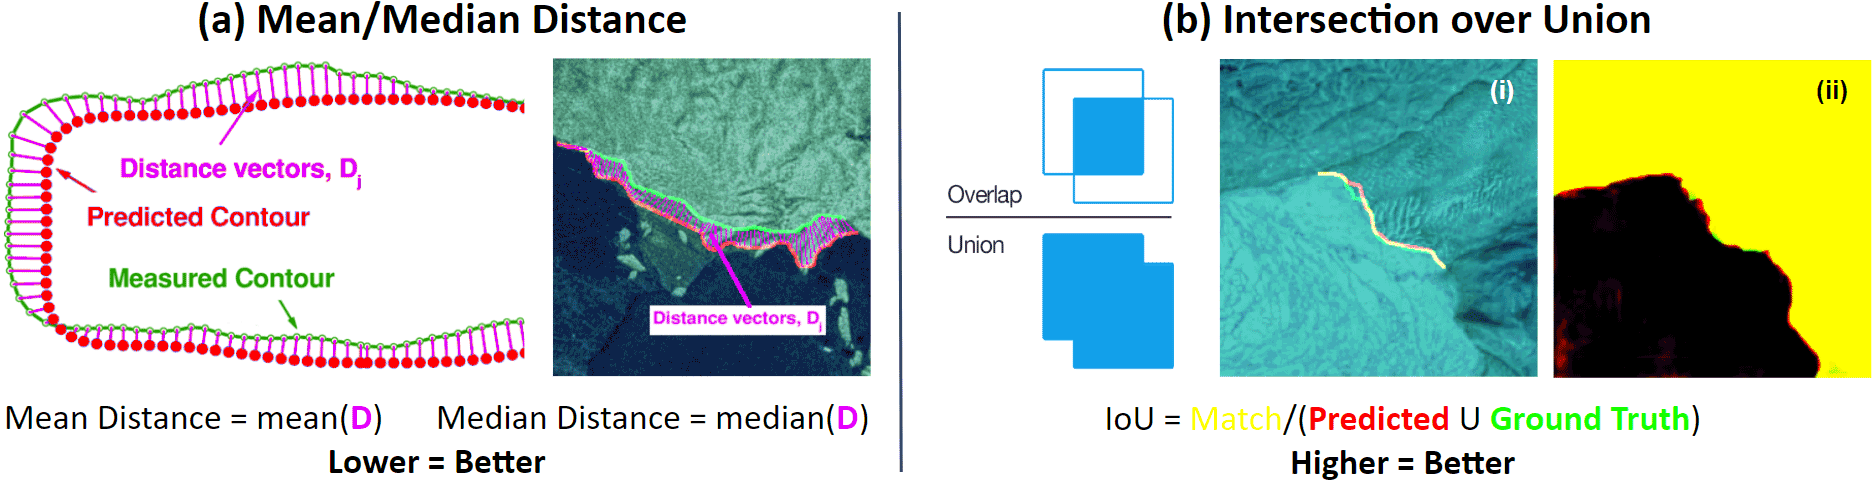
\includegraphics[width=17cm]{figures/qa_example.png}
    \centering
    \caption{A visual outline of Mean/Median Distance Error Estimation (a) and Classification Accuracy with Intersection over Union (b). (b.i) and (b.ii) show the evaluation of IoU on the primary calving front and secondary ice/ocean mask CALFIN outputs, respectively.}
    \label{fig:error_analysis}
\end{figure}
%Image sources:
%MDE: https://www.spiedigitallibrary.org/journals/Journal-of-MicroNanolithography-MEMS-and-MOEMS/volume-9/issue-4/041302/Alignment-and-averaging-of-scanning-electron-microscope-image-contours-for/10.1117/1.3514704.short
%IoU: https://www.pyimagesearch.com/2016/11/07/intersection-over-union-iou-for-object-detection/

\subsection{Error Estimation}
\label{sec:error_estimation}
The first quality assessment method is the Mean Distance Error. This metric is used by Mohajerani et al., Zhang et al., and Baumhoer et al. This metric evaluates the average distance between closest points between predicted and manually delineated calving fronts. Conceptually, this method resembles numerical integration of the area between two curves, normalized by the average length of the curves (see Figure \ref{fig:error_analysis}a). This method can also be seen as a generalization of the method of transects along arbitrarily oriented fronts \citep{mohajerani2019, baumhoer2019}. This metric is implemented by averaging the distance between closest pixels in the predicted and ground truth fronts.

\setlength{\intextsep}{12.0pt plus 2.0pt minus 2.0pt}

\subsection{Classification Accuracy}\label{sec:classification}
The second quality assessment method calculates the Intersection over Union, or Jaccard index. This is one of the metrics used by Baumhoer et al. This metric evaluates the degree of overlap between the predicted and ground truth pixel masks of the calving front. It is calculated by dividing the number of pixels in the intersection of two masks over the number of pixels in the union of the two masks (see Figure \ref{fig:error_analysis}b). When calculating the IoU between 3 pixel wide edges, this measure is very conservative: 1 pixel of difference results in a score of 0.5000, and scores in that range and above are indicative of human levels of accuracy. When calculating the IoU between large land/ice-ocean-mélange masks, this measure is less conservative, and scores in the range of 0.9000 and above are indicative of human levels of accuracy.

\subsection{Validation Results}
\label{sec:validation_results}
The following subsections list tables that print the above metrics for the associated validation sets, the values from the original studies, and a subset of the outputs of CALFIN on each.

Our primary validation set, the CALFIN validation set, consists of 162 images with clouds, illumination differences, ice mélange, and Landsat 7 Scanline Corrector Errors (L7SCEs). This set contains data from 66 Greenlandic basins, including data from Helheim, which was specifically excluded from CALFIN's training set for validation purposes - as done by Mohajerani et al. This set ensures CALFIN produces consistent results on new data, and addresses concerns raised by Zhang et al. section 7.3 regarding issues of applying this method to new data. We also evaluate two validation subsets, CALFIN-L7SCE-only/none, which isolate and exclude images with L7SCEs, respectively.

To allow for model inter-comparisons, we additionally output CALFIN's performance on previous studies' validation sets, where appropriate. These include the 10 Landsat Helheim subsets used in Mohajerani et al., the 6 TerraSAR-X Jakobshavn subsets used in Zhang et al., and 62 Sentinel-1 Antarctic domains taken from the 11 validation scenes used in Baumhoer et al.

\setlength{\intextsep}{4.0pt plus 2.0pt minus 2.0pt}

\subsubsection{CALFIN Validation Set}
\label{sec:calfin_val}
CALFIN performs well on the CALFIN validation set. We achieve a mean distance error of 2.25 pixels, or approximately 87.76 meters. When including only images with L7SCEs (CALFIN-L7SCE-only), the error changes to 2.22px (91.93m), showing CALFIN's robustness to L7SCEs. A decrease in mean pixel distance and an increase in Calving Front IoU are explained by the L7SCE images having a generally higher meter per pixel ratio. When excluding outliers such as Kong-Oscar, the median distance error drops to a very accurate 1.21px (44.59m). Given that the nominal pixel scale of Landsat 5-8 imagery is 30 meters, this error is on the order of human levels of variance. Assuming that the validation set of 162 images is a representative sample of our 14000 source images, we calculate our margin of error at 99.5\% confidence to be 2.36\%. In other words, the true mean distance error of our automatically generated calving fronts is 99.5\% likely to be within 86.76 $\pm$ 2.05m.

\begin{table}[H]
    %\caption{A subset of outputs from CALFIN running on the CALFIN validation scenes.}
    \centering
    \setlength{\extrarowheight}{0pt}
    \addtolength{\extrarowheight}{0.5pt}
    \addtolength{\extrarowheight}{0.5pt}
    \setlength{\aboverulesep}{0pt}
    \setlength{\belowrulesep}{0pt}
    \begin{tabular}{cccccc} 
    \toprule
    \rowcolor[rgb]{0.71,0.71,0.71} Validation Set & Model & Mean Distance & Median Distance & IoU Calving Front & IoU Ice/Ocean \\ 
    \hline\hline
    CALFIN & CALFIN & 2.25px, 86.76m & 1.21px, 44.59m & 0.4884 & 0.9793 \\
    \hline
    \rowcolor[rgb]{0.886,0.886,0.886} CALFIN-L7SCE-none & CALFIN & 2.27px, 81.65m & 1.16px, 44.01m & 0.4880 & 0.9819 \\
    CALFIN-L7SCE-only & CALFIN & 2.22px, 91.93m & 1.33px, 49.24m & 0.4888 & 0.9766 \\
    \bottomrule
    \end{tabular}
    \label{tab:validation_calfin}
\end{table}

\begin{figure}[H]
    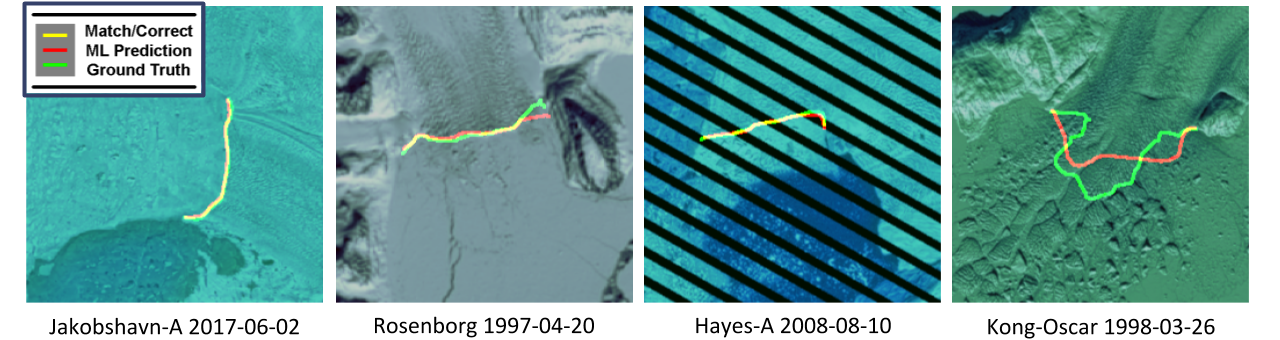
\includegraphics[width=13.5cm]{figures/validation_calfin.png}
    \centering
    \caption{A subset of CALFIN validation outputs. Yellow represents human (green) and machine (red) agreement on the front location.}
    \label{fig:validation_calfin}
\end{figure}


\subsubsection{Mohajerani et al. Validation Set}
\label{sec:mohajerani_val}
CALFIN performs well on the Mohajerani validation set. This demonstrates the generalization capability of the CALFIN network, which improves upon Mohajerani et al. This is further supported by the results of the model inter-comparison described in Section \ref{sec:intercomp}. Note that Mohajerani et al. does not provide ice/ocean mask data, so it was not evaluated.

\begin{table}[H]
    %\caption{Evaluation metrics for CALFIN and Mohajerani on the Mohajernai validation set. Note that Mohajerani et al. does not provide ice/ocean mask data, so it was not evaluated.}
    \centering
    \setlength{\extrarowheight}{0pt}
    \addtolength{\extrarowheight}{0.5pt}
    \addtolength{\extrarowheight}{0.5pt}
    \setlength{\aboverulesep}{0pt}
    \setlength{\belowrulesep}{0pt}
    \begin{tabular}{cccccc} 
    \toprule
    \rowcolor[rgb]{0.71,0.71,0.71} Validation Set & Model & Mean Distance & Median Distance & IoU Calving Front & IoUIce/Ocean \\ \hline\hline
    Mohajerani & CALFIN & 2.56px, 97.72m & 2.55px, 97.44m & 0.3332 & N/A \\
    \rowcolor[rgb]{0.886,0.886,0.886} Mohajerani & Mohajerani & 1.97px, 96.31m & N/A & N/A & N/A \\ 
    \bottomrule
    \end{tabular}
    \label{tab:mohajerani}
\end{table}

\begin{figure}[H]
    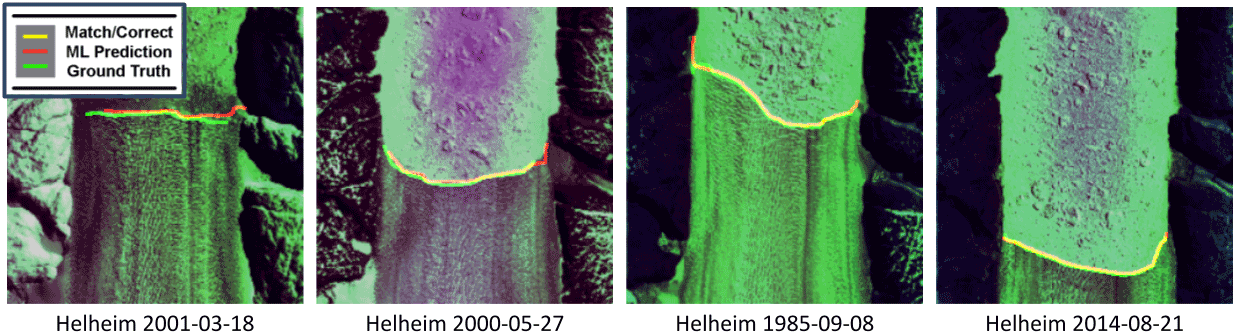
\includegraphics[width=13.5cm]{figures/validation_mohajerani.png}
    \centering
    \caption{Mohajerani et al. validation outputs subset. Note that CALFIN-NN has never trained on Helheim, but can still predict the front at multiple scales and conditions.}
    \label{fig:mohajerani}
\end{figure}


\subsubsection{Zhang et al. Validation Set}
\label{sec:zhang_val}
CALFIN does performs adequately on the Zhang validation set. We note that despite being SAR data and being restricted to using lower resolution QuickLook subsets, we still achieve a better per-pixel accuracy measure than Zhang et al (3.56px vs. 17.3px). Exclusion of outliers results in a median distance error of 1.69px (114.50m), which is on par with the accuracy achieved on CALFIN Jakobshavn validation images (90.39m). We posit that increasing CALFIN-NN's input resolution, testing on higher resolution SAR data, and additional training will enable CALFIN to perform better. 

\begin{table}[H]
    \centering
    \setlength{\extrarowheight}{0pt}
    \addtolength{\extrarowheight}{0.5pt}
    \addtolength{\extrarowheight}{0.5pt}
    \setlength{\aboverulesep}{0pt}
    \setlength{\belowrulesep}{0pt}
    \begin{tabular}{cccccc} 
    \toprule
    \rowcolor[rgb]{0.71,0.71,0.71} Validation Set & Model & Mean Distance & Median Distance & IoU Calving Front & IoUIce/Ocean \\ 
    \hline\hline
    Zhang & CALFIN & 3.56px, 284.22m & 1.69px, 114.50m & 0.3739 & 0.9778 \\
    \rowcolor[rgb]{0.886,0.886,0.886} Zhang & Zhang & 17.3px, 104m & N/A & N/A & N/A \\ 
    \bottomrule
    \end{tabular}
    \label{tab:zhang}
\end{table}

\begin{figure}[H]
    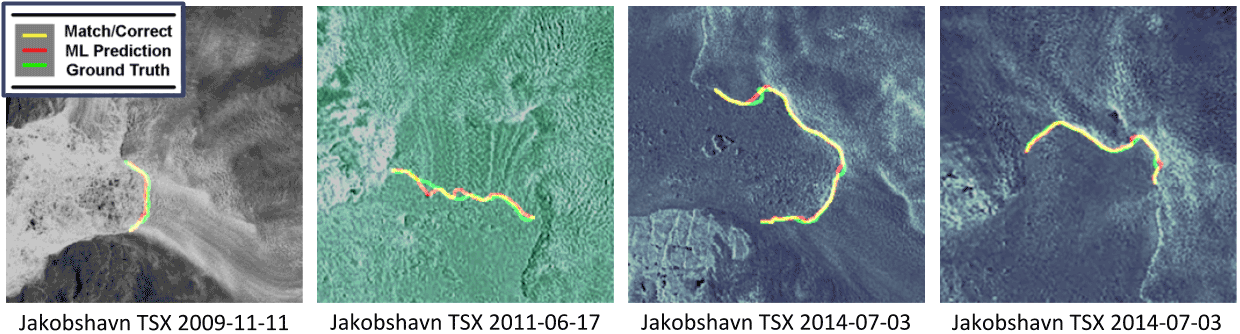
\includegraphics[width=13.5cm]{figures/validation_zhang.png}
    \centering
    \caption{A subset of outputs from CALFIN running on validation scenes from Zhang et al.}
    \label{fig:zhang}
\end{figure}


\subsubsection{Baumhoer et al. Validation Set}
\label{sec:baumhoer_val}

CALFIN performs sub-par on the Baumhoer validation set, though this is admissible as the set consists of Antarctic SAR imagery. Additionally, we do not include static coastlines, which would otherwise lower our mean distance error. Currently, our mean distance error is skewed by deviations in the kilometer range by a combination of very large domains, and the fact that CALFIN-NN was not trained to reliably detect calving fronts at such large scales. After excluding such outliers, we achieve median distance errors of 0.95px (127.87m), which is consistent with our expectations when generalizing to new SAR data.

\begin{table}[H]
    \centering
    \setlength{\extrarowheight}{0pt}
    \addtolength{\extrarowheight}{0.5pt}
    \addtolength{\extrarowheight}{0.5pt}
    \setlength{\aboverulesep}{0pt}
    \setlength{\belowrulesep}{0pt}
    \begin{tabular}{cccccc} 
    \toprule
    \rowcolor[rgb]{0.71,0.71,0.71} Validation Set & Model & Mean Distance & Median Distance & IoU Calving Front & IoUIce/Ocean \\ 
    \hline\hline
    Baumhoer & CALFIN & 3.36px, 543.47m & 0.95px, 127.87m & 0.5959 & 0.9873 \\
    \rowcolor[rgb]{0.886,0.886,0.886} Baumhoer & Baumhoer & 2.69px, 108m & N/A & N/A & 0.905 \\
    \bottomrule
    \end{tabular}
    \label{tab:baumhoer}
\end{table}

\begin{figure}[H]
    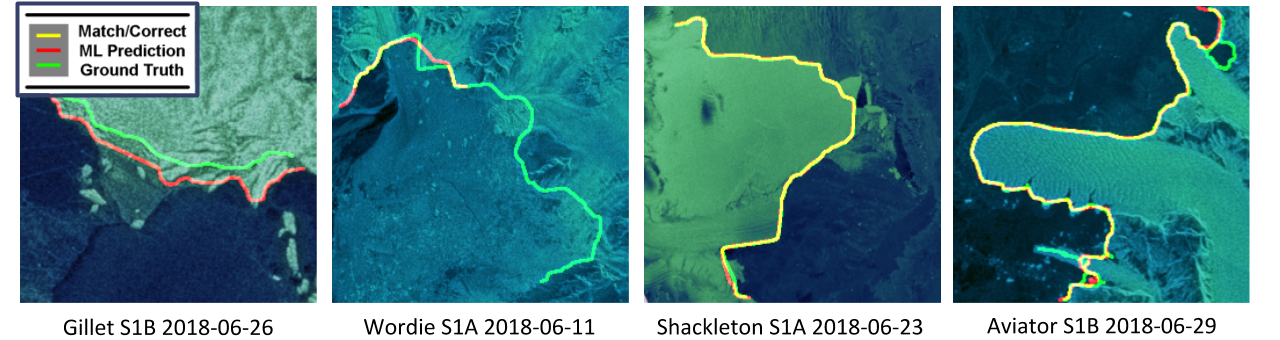
\includegraphics[width=13.5cm]{figures/validation_baumhoer.png}
    \centering
    \caption{A subset of outputs from CALFIN running on validation scenes from Baumhoer et al.}
    \label{fig:baumhoer}
\end{figure}

\setlength{\intextsep}{12.0pt plus 2.0pt minus 2.0pt}


\subsection{Detection Accuracy}
\label{sec:accuracy}
Lastly, we show that CALFIN-NN has the ability to automatically filter images that do not have visible calving fronts. To verify this, we include 13 images in the test set which contain adverse image conditions, and thus do not contain discernible calving fronts. We calculate the true positive, true negative, false positive, and false negative rates for the entire 162 image data set, and output the confusion matrix below. We note that CALFIN-NN does not output any false positives on our validation set. This behavior is desired, as it ensures we output fronts conservatively, rather than output incorrect fronts.

\begin{table}[h]
	\centering
	\caption{Confusion matrix showing CALFIN-NN's ability to not only detect fronts in images, but discern whether there are any fronts at all.}
	\label{confusion-matrix}
	\begin{tabular}{c|c|c|c|}
		\multicolumn{1}{c}{} & \multicolumn{1}{c}{} &  \multicolumn{2}{c}{Front Detected?} \\ 
		\cline{3-4}
		\multicolumn{1}{c}{} &  & \rowcolor[rgb]{0.71,0.71,0.71} Yes & No \\ 
		\cline{2-4}
		\multirow{2}{*}{Front Exists?} & \cellcolor[rgb]{0.71,0.71,0.71} Yes & TPR = 141/149 = 94.63\% & FNR = 8/139 = 5.76\% \\ 
		\cline{2-4}
		& \cellcolor[rgb]{0.71,0.71,0.71} No & FPR = 0/13 = 0.00\% & TNR = 13/13 = 100.00\% \\
		\cline{2-4}
	\end{tabular}
	\label{tab:confusion_matrix}
\end{table}

\section{Results}
\label{sec:results}
We generate results that are two-fold in nature. First, we release the calving front data we produced throughout the study. Secondly, we release an implementation of CALFIN-NN to the scientific community for use, study, and further development.

\subsection{CALFIN Dataset}
\label{sec:results_dataset}

\begin{figure}[h]
    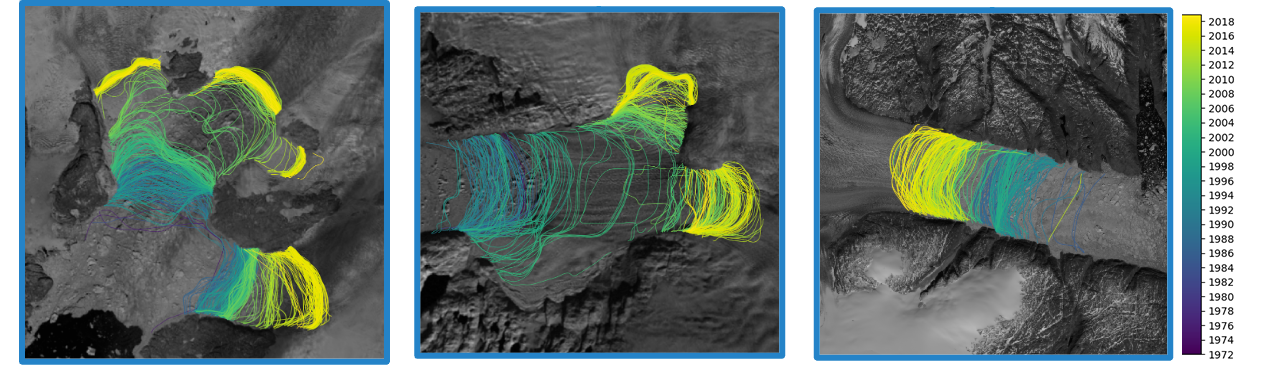
\includegraphics[width=17cm]{figures/results_with_legend.png}
    \centering
    \caption{A sample of CALFIN's dataset, shown for Upernavik (left), Jakobshavn (center), and Helheim (right).}
    \label{sec:timeseries}
\end{figure}

We release the CALFIN dataset, which spans 67 Greenlandic glaciers, over the period 1972-2019. This consists of over 1600 manual delineations and over 20000 automatically delineated calving fronts.

We provide 2 levels of CALFIN data products.

Level 0 products include the raw inputs and basic outputs used for CALFIN-NN. These products consist of the raw GeoTiff domain subsets, the domain Shapefiles used for subsetting, neural network pixel mask outputs, and a quality assurance image for validation purposes. Use cases of Level 0 products may include studies of reproducibility, validation, or training new neural networks.

Level 1 products includes the calving front polyline and polygon Shapefiles. The polyline product consists of the isolated, refined, and geo-referenced calving fronts for each domain. The polygon product consists of an ocean mask bounded by the domain subset bounds, the fjord boundaries, and the calving front, for each domain. Shapefiles are projected to EPSG:3413.

\subsection{CALFIN-NN Implementation}
\label{sec:results_implementation}
We release an implementation of CALFIN-NN, including the weights and architecture we develop throughout this study. It is our intention that any innovations as described in Section \ref{sec:proc} can be applied to other networks and applications. The implementation is written in Python 3, and open access to the code is available at on Github. For access to the network weights/parameters, please see the associated link on Google Drive. For additional details regarding the training, see the following Discussion sections \ref{sec:training_data}-\ref{sec:training_regimen}.


\section{Discussion}
\label{sec:discussion}
\subsection{CALFIN-NN Training Data}
\label{sec:training_data}
In order to train our network, we create training data, which consists of preprocessed inputs and ground truth images. Our primary training data consists of 1703 images pairs, with 1541 pairs for training and 162 pairs for validation. We additionally add 232 training pairs consisting of Antarctic SAR data extracted from the same training scenes used by Baumhoer et al. This data was made manually in order to ensure consistency and quality in the delineations. The training data has the secondary purpose of providing trustworthy delineations for the CALFIN database, and the calving front masks are output as part of the data release. Raw training images are stored in 16-bit unsigned integer (uint16) RGB images, masks are formatted as uint16 greyscale images, and GeoTIFF subsets are converted to uint16 from their native formats.

\subsection{CALFIN-NN Training Regimen}
\label{sec:training_regimen}
We trained the network over 80 epochs, with 4000 batches per epoch, and 8 images per batch. We utilized a K40 Nvidia Tesla GPU, with each epoch taking about 126 minutes to complete, and about 1 week to complete all 80 epochs. The optimal final network weights were taken from the 65th training epoch. We utilize the Adam optimizer, which automatically computes optimal learning rates per parameter. Our Adam optimizer is modified to accumulate the gradient over 2 batches, so that our effective batch size is 16. Additionally, it clips the learning rate at 1e-4, to prevent exploding gradients during training.
We utilize Exponential Linear Units (ELU) over ReLU as our activation function, to prevent vanishing gradients. Our loss function is a weighted combination of binary cross entropy (BCE) and two Intersection-over-Union (IoU) calculations. 
This loss function heavily penalizes incorrect predictions (a property of BCE/IoU), heavily favors correct predictions (a property of IoU), and is differentiable (a property of the natural logarithm). Additionally, the weighting heavily favors correct coastline/edge mask predictions, which is critical for increasing calving front positional accuracy.

\subsection{CALFIN-NN Data Augmentation/Test-time Augmentation}
\label{sec:augmentation}
To avoid overfitting our model, we used data augmentation to generate new inputs from our existing training sets. These augmentations include random flips/transpositions, random Gaussian noise, random sharpen filters, random rotations of up to 12°, random crops, and random scaling. Together, these alterations ensure a greater diversity of data, while still ensuring that the network could train on a fully continuous calving front. We determined through empirical testing that excessive image padding, rotation, non-affine warping, and partially clipped calving fronts resulted in sub-optimal performance.

We also utilize test-time augmentations to enhance detection accuracy and confidence. We use 9 overlapping 224x224 windows, and reassemble them into the final 256x256 output mask. Edge artifacts remain visible in the output masks, but are rendered inconsequential during postprocessing.

\subsection{Existing Work}
\label{sec:existing}
Mohajerani et al. provides a similar case study using the same type of deep neural network architecture to detect calving fronts. The study is performed on the Greenlandic glacial basins Jakobshavn, Helheim, Sverdrup, and Kangerlussuaq. Mohajerani's methodology is restricted in its preprocessing requirements and ability to handle branching/non-linear calving fronts, but nonetheless displays promising steps towards generalizability of the neural network method.

Zhang et al. performs an analysis similar to Mohajerani, albeit in a more specific case study using SAR data of Jakobshavn. While limited in scope, the applicability of neural networks as a general methodology for calving front analysis is supported by its successful usage.

Baumhoer et al. evaluates modified UNet architectures, as applied to SAR data of Antarctica. The study incorporates large spatial context in order to capture whole-coastline delineations. The prospect of larger networks on the order of 768x768 pixels offers the promise of higher resolution/accuracy outputs.

Our methodology shares the same basic approach with the above. We utilize an updated neural network architecture - DeeplabV3+ Xception - that improves upon the base UNet design. Furthermore, we use additional training data and post-processing steps to make the detection more accurate.

\subsection{Inter-model Comparison}
\label{sec:intercomp}
We conduct a comprehensive inter-model comparison between CALFIN and the model developed by Mohajerani et al. To perform this task, we process the validation data used by each other's models, and compare the results.

\begin{table}[h]
    \centering
    \caption{Consolidated accuracy and error metrics for CALFIN and Mohajerani on each other's validation sets. Note the 2nd row where we evaluate a retrained Mohajerani model.
    }
    \setlength{\extrarowheight}{0pt}
    \addtolength{\extrarowheight}{\aboverulesep}
    \addtolength{\extrarowheight}{\belowrulesep}
    \setlength{\aboverulesep}{0pt}
    \setlength{\belowrulesep}{0pt}
    \begin{tabular}{cccccc} 
    \toprule
    \rowcolor[rgb]{0.71,0.71,0.71} Validation Set & Model & Mean Distance & Median Distance & IoU Calving Front & IoUIce/Ocean \\ 
    \hline\hline
    CALFIN & CALFIN & 2.25px, 86.76m & 1.21px, 44.59m & 0.4884 & 0.9793 \\
    \rowcolor[rgb]{0.886,0.886,0.886} CALFIN & Mohajerani & 4.45px, 201.35m & 1.25px, 50.52m & 0.4935 & 0.9699 \\ 
    \hline
    Mohajerani & CALFIN & 2.56px, 97.72m & 2.55px, 97.44m & 0.3332 & N/A \\
    \rowcolor[rgb]{0.886,0.886,0.886} Mohajerani & Mohajerani & 1.97px, 96.31m & N/A & N/A & N/A \\ 
    \bottomrule
    \end{tabular}
    \label{tab:intercomp}
\end{table}

%\begin{figure}[t]
%\includegraphics[width=15cm]{figures/helheim_plots_intercom%p.png}
%\caption{Validation test for 1 of the 10 images used in %Mohajerani et al. \textbf{b)} is an RGB image containing %the raw image (R), a High Dynamic Range toned image (G), %and a Shadows/Highlights enhanced image (B). \textbf{c)} is %the RGB output of CALFIN-NN, containing the coastline/edge %mask (R) and the land-ice/ocean mask (G). \textbf{e)} %compares the fronts from our method (R), the ground truth %(G), and Mohajerani et al. (B). The Jaccard index %calculates the overlap between our method and the ground %truth as a percentage from 0 to 1. \textbf{f)} is a %histogram that shows the distribution of distances between %points in CALFIN's predicted front and the ground %truth.}
%\centering
%\end{figure}

Across all 162 test images in the CALFIN validation set, CALFIN-NN attains a 2.25 pixel (86.76 meter) mean distance between the predicted and the ground truth fronts. This exceeds the level of accuracy achieved by the model from Mohajerani et al., which after retraining on CALFIN training data, was 4.45 pixels (201.35 meters). Note that Landsat 7 images were excluded during reevaluation for the model from Mohajerani et al. This supports our findings that the CALFIN-NN architecture is an improvement over existing models.

Across all 10 test images in the Mohajerani et al. validation set, CALFIN-NN attains a 2.56 pixel (97.72 meter) mean distance between the predicted and the ground truth fronts. This approaches the level of accuracy achieved in the original study, which was 1.97 pixels (96.31 meters). This supports our findings that CALFIN-NN architecture generalizes to new data well. Note that CALFIN's larger network size requires additional training data to avoid overfitting, which could explain the slightly lesser accuracy when compared to the model from Mohajerani et al.

Furthermore, we note that \citep{mohajerani2019} obtained the mean error estimate by breaking each delineated front to 1000 smaller segments within a small buffer from the fjord walls and calculating the mean deviation between the segments of the true and delineated fronts. Here we calculate the errors by getting the mean distance between each pixel of the delineated front and the closest pixel of the true front. This does not require the fronts to have the same number of pixels, as several pixels can be mapped onto one pixel. It is important to emphasize that the error results can be very sensitive to the error evaluation methodology. By comparing pixels directly, we avoid comparing line segments far from each other due to different lengths of the delineated and true fronts. In that sense, the line-segment methodology of \citep{mohajerani2019} provides a more conservative estimate as it relies on line segments being close to each other.

Overall, this inter-comparison supports the hypothesis that our methodology improves upon existing studies and is generalizing well.

\conclusions[Conclusion \& Future Work]
\label{sec:conclusion}
The calving front data products are being released on NSIDC. %datadryad or NSIDC?
The neural network model is being released on Github, accessible at \url{https://github.com/daniel-cheng/CALFIN}.

Overall, we accomplish our goal of automatically delineating calving fronts from satellite imagery. Our method utilizes the cutting-edge in deep learning architectures. Our method is robust to minor cloud cover, Landsat 7 Scanline Corrector Errors, and illumination changes. We address issues with generalization through use of additional training data and an improved neural network architecture.

Future work may entail accuracy improvements, expansion of included domains, usage of SAR data sources, and near-real time data products. Within the community, we anticipate the benefit of standardized training, and validation sets, and outputs/metadata. We also anticipate the community's development of new automated extraction studies, such as grounding line delineation, iceberg tracking, and sea ice mélange measurements.

Ultimately, this work showcases the state-of-the-art in automated calving front detection, and provides a new database of glacial termini positions for the cryosphere community.


\codedataavailability{
    The code used to automate the CALFIN pipeline is freely available here: https://github.com/daniel-cheng/CALFIN
    
   The data generated by CALFIN, including Level 0 and 1 data products, are freely available here: (NSIDC link)
}

\supplement{.pdf}

\authorcontribution{
    D. Cheng developed the code/model, created the training data, carried out the data processing, and wrote majority of the manuscript.
    W. Hayes provided direction on the processing methodology, post-processing algorithms, and error analysis.
    E. Larour provided key direction for the overall study and outputs.
    Y. Mohajerani performed the model inter-comparison and assisted with the writing of the manuscript.
    MW assisted with the model inter-comparison.
    I. Velicogna assisted in organizing collaborators and model inter-comparison.
    M. Wood performed the data preprocessing for the model inter-comparison.
    E. Rignot contributed suggestions regarding the error analysis and inter-comparison.
    W. Hayes, E. Larour, I. Velicogna, and E. Rignot reviewed the manuscript and evaluated the results.
}

\competinginterests{
    The authors declare no competing interests.
}

\begin{acknowledgements}
    This work was conducted as a collaboration between NASA’s Jet Propulsion Laboratory and the University of California, Irvine. 
\end{acknowledgements}

\bibliographystyle{copernicus}
\bibliography{references.bib}  %%% Use the external .bib file (using bibtex).

\end{document}